\section{Additional Test Results and Robustness Checks}
\label{app:completed_results}

\subsection{Additional test sets for the same four domains}
\label{app:independent_domain_test}

The ten joint-training configurations use the development benchmarks and checkpoint grid in Appendix~\ref{app:setup}. The following analyses evaluate selected checkpoints on separate test questions, measure candidate-set coverage, and check sensitivity to known training--evaluation overlap.

The separate-test means in Table~\ref{tab:main_outcomes} use 256 additional questions per domain: 1,024 questions and 1,792 responses per model. Mathematics and code come from the Skywork-OR1-RL-Data mathematics and TACO-based code pools; instruction following uses Nemotron-RL-instruction\_following; science uses the Nemotron-RL-knowledge-mcqa validation split restricted by a fixed natural-science keyword filter. Questions are the first eligible unique candidates in the fixed source order. Normalized exact-match and lexical near-duplicate checks remove questions matching the original training bundle or known evaluation pools.

Scoring uses mathematics answer verification, code unit tests, instruction-following constraints, and science multiple-choice accuracy. Mathematics, code, and instruction following use greedy decoding; science uses four responses per question at temperature 1. The context budget is 32,768 tokens, with thinking disabled. The four-domain mean weights domains equally. Question-paired bootstrap intervals quantify finite-test uncertainty.

\subsection{Checkpoint selection before test evaluation}
\label{app:completed_selection}

We apply the three selection rules in Section~\ref{sec:recipe} to the development grid in Appendix~\ref{app:setup}. The grid contains updates 50/100/250/500 for seven Adam trajectories and 100/250/500 for three SGD trajectories. The retention tolerance is two percentage points per domain relative to the initial student. Both development rules keep the initial student unless the selected equal-domain mean improves by at least one percentage point. Both development-based rules choose update 250 for PG-DT/Adam and update 500 for the other nine trajectories. The separate PG-DT/Adam update-250 test evaluation allows direct comparison with its update-500 endpoint.

The development grid contains 37 trained-checkpoint evaluations along the same ten trajectories, including the ten endpoints reported in Table~\ref{tab:main_outcomes}.

The retention-constrained and maximum-mean rules select the same checkpoint in every trajectory. On the additional test sets, the update-250 PG-DT/Adam checkpoint scores 0.37 percentage points below its update-500 endpoint in four-domain mean. The endpoint therefore has the higher separate-test mean in this comparison. PG-DR/Adam has two intermediate development checkpoints outside the retention tolerance: GPQA falls from 32.20\% initially to 28.03\% at update 50 and 30.18\% at update 250, before reaching 35.97\% at update 500. The learning curve captures these temporary regressions and their subsequent recovery.

\subsection{Probability mass retained by the candidate intersection}
\label{app:actual_intersection_coverage}

For each of four student checkpoints (M-PG and M-I64-DR at updates 100 and 500), four cached response batches provide one response per domain and six sampled positions per response: 96 prefixes per checkpoint. Each response is scored by its domain teacher. We measure $p_\theta(I\mid h)$ for the actual intersection $I=S\cap T$ and the retained fraction $r=p_\theta(I\mid h)/p_\theta(S\mid h)$.

Mean student probability mass in the actual student--teacher top-64 intersection exceeds 99.9\% at each of the four checkpoints. The minimum over the 384 sampled prefixes is 96.55\%, and no intersection is empty.

\subsection{Sensitivity to known mathematics overlap}
\label{app:math_overlap_sensitivity}

The fixed Qwen training pool contains five records matching four known MATH-500 problems, including variants in wording or answer format. The affected MATH test identifiers are counting-and-probability problem 430 and intermediate-algebra problems 1849, 2146, and 582. We remove these four questions from the existing per-question evaluation results, retaining the original 500-question results as the main protocol.

Removing the four questions changes the four-domain means by approximately 0.09--0.16 points and can reorder near-tied configurations. PG-DT/Adam and PG-GT/Adam both round to 38.60\% before removal, but reach 38.70\% and 38.75\%, respectively, afterward. PG-DR/SGD retains the highest mean among the reported checkpoints. MATH-496 denotes this retained subset of MATH-500.

\subsection{Teacher-update overlap and distributional similarity}
\label{app:teacher_overlap_support}

\begin{figure}[!htbp]
\centering
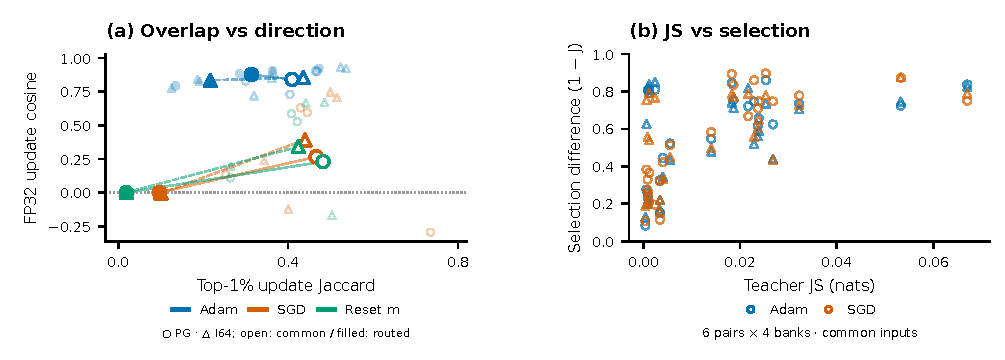
\includegraphics[width=\linewidth]{figures/nine_panel_20260914/appendix_teacher_overlap.pdf}
\caption{\textbf{Coordinate overlap and update direction measure different properties.}
(a) Top-1\% FP32 update-set Jaccard versus cosine; small/large points show batch/overall means.
(b) Teacher-distribution JS divergence versus $1-$Jaccard on shared inputs; each point is a teacher pair within a batch.}
\label{fig:teacher_overlap_support}
\end{figure}

Figure~\ref{fig:teacher_overlap_support} supplements the zero-gradient baseline subtraction at M-PG/500 using the controls in Appendix~\ref{app:nine_panel_support}. It compares PG and I64 under Adam with trained moments, reset-$m$, and norm-matched SGD. Shared inputs hold student prefixes fixed between teachers; domain-specific inputs change both the teacher and the input domain. Each of four batches contains six teacher pairs.

\FloatBarrier
\subsection{Online coverage and per-domain normalization effects}
\label{app:i16_online_coverage}
\label{app:domain_probe_breakdown}

\paragraph{Online I16 coverage.}
For I16-DR, each of 500 updates has 16 logged slices of four responses. Each update averages the masked, response-averaged summaries with equal weight per slice. Candidate sets are fixed at rollout; student probabilities are measured during training. Across 8,000 slices, mean $p_\theta(I)$, $r$, and $|I|$ are 99.62\%, 99.88\%, and 15.05. The mean empty fraction is 0.0027\%, nonzero in 80 slices across 62 updates. The lowest slice-mean mass is 86.67\% and largest slice-mean empty fraction 1.85\%; these extremes refer to slice means.

\paragraph{Per-domain probe losses.}
We disaggregate Figure~\ref{fig:normalization_interventions}(c), using the same six batches and twelve branches per batch (Appendix~\ref{app:fixed_batch_normalization}). Each batch has one held-out response per domain. At update 250, saved-state Adam under DR/DT/GT increases IF KL by $0.362/0.293/0.272\times10^{-3}$, while the four-domain changes are $0.041/-0.002/-0.027\times10^{-3}$. Thus the mean reduction under DT/GT coexists with an instruction-following increase.

\begin{figure}[!htbp]
\centering
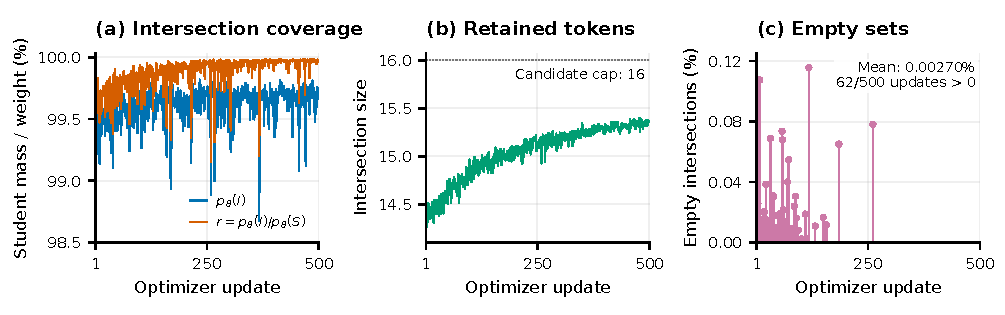
\includegraphics[width=\linewidth]{figures/coverage_domain_controls_20260917/i16_online_coverage.pdf}
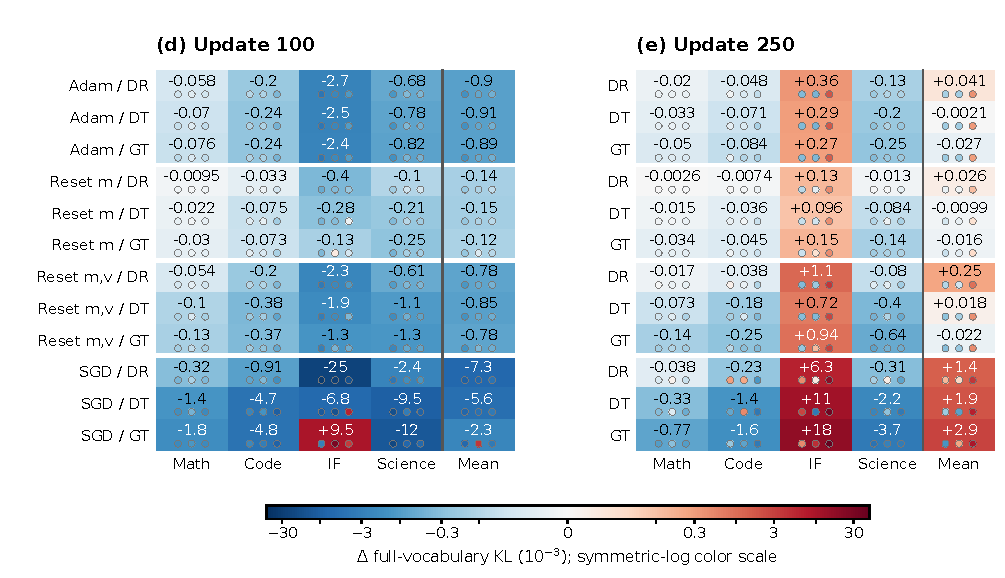
\includegraphics[width=\linewidth]{figures/coverage_domain_controls_20260917/normalization_domain_probe.pdf}
\caption{\textbf{High average coverage and low mean probe loss can conceal exceptions.}
(a--c) I16 per-update means of 16 logged slices, without temporal smoothing; the mass axis spans 98.5--100\%.
(d,e) Full-vocabulary KL after minus before BF16 writeback, in units of $10^{-3}$. Cells show three-batch means; dots show batches 1042--1044 from left to right. The shared symmetric-log color scale is linear within $\pm0.1$. SGD is matched to each rule's Adam step norm.}
\label{fig:coverage_domain_controls}
\end{figure}
